\chapter{Model Architecture}
\label{ch:model-architecture}

\section{Offline v4 Research Architecture}

The offline v4 system was the strongest research configuration before the
project moved from the IndustReal benchmark to the internally collected
engine-model dataset. It established the representation that was retained in
the later deployment: two complementary, frozen video encoders whose outputs
are normalized and fused. Its temporal and correctness heads, however, were
designed for complete recordings and could use context from both sides of a
transition. It was therefore an important research reference and an upper
bound, rather than the final live architecture.

\begin{figure}[H]
\centering
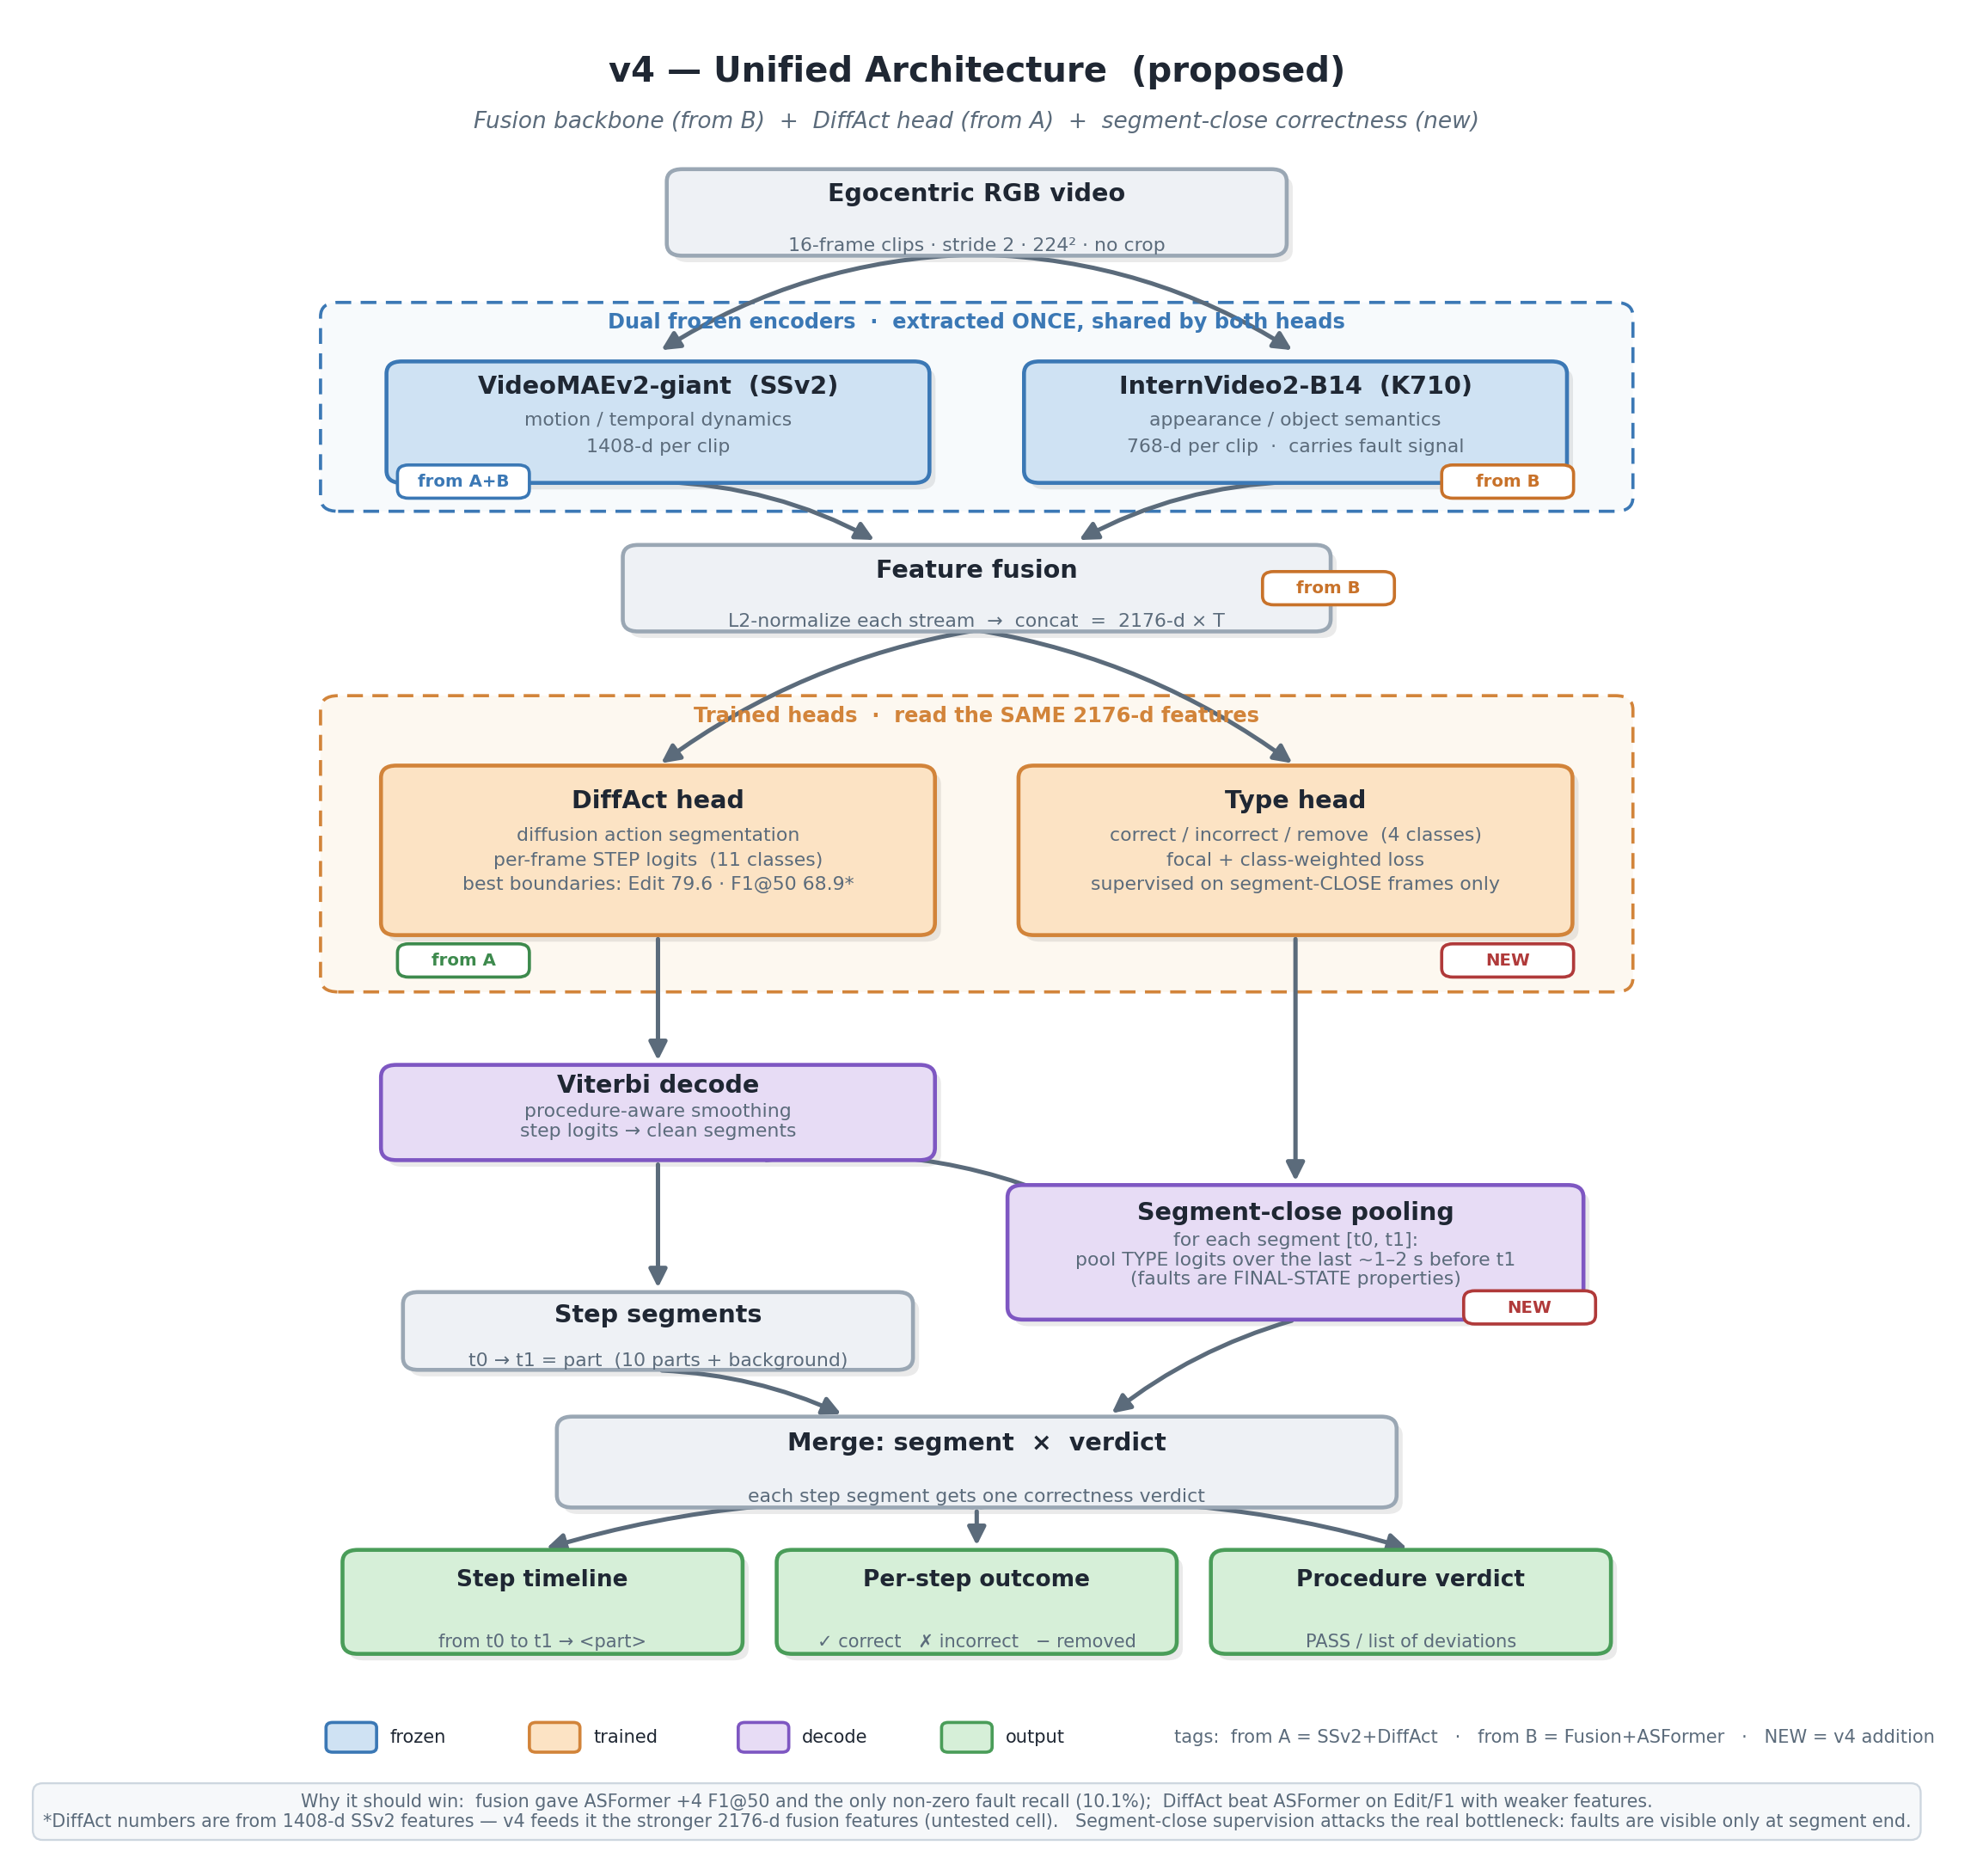
\includegraphics[width=0.88\textwidth]{architecture_v4.png}
\caption{Offline v4 research architecture: fused motion and appearance
features feed the DiffAct segmentation head, type reasoning, and Viterbi
decoding before segment-level outcomes are produced.}
\label{fig:offline-v4-architecture}
\end{figure}

The offline pipeline can be read from left to right. VideoMAEv2-giant provides
the motion-sensitive representation and InternVideo2-B14 provides a
complementary appearance representation. Their 1,408- and 768-dimensional
outputs form a 2,176-dimensional sequence feature. DiffAct predicts the
temporal action structure, while the type head provides an additional signal
for segment interpretation. Viterbi decoding then imposes temporal
consistency and closes segments before a verdict is emitted.

\begin{table}[H]
\centering
\small
\begin{tabularx}{\textwidth}{@{}p{0.32\textwidth}X@{}}
\toprule
\textbf{Offline component} & \textbf{Purpose} \\
\midrule
VideoMAEv2-giant & Frozen motion and temporal-dynamics representation; 1,408
dimensions per clip. \\
InternVideo2-B14 & Frozen appearance and object-semantic representation; 768
dimensions per clip. \\
Feature fusion & L2-normalize both streams and concatenate them into a
2,176-dimensional sequence feature. \\
DiffAct head & Offline action-segmentation head producing per-frame step
logits and strong segment-boundary evidence. \\
Type head and segment close & Exploratory correctness/type reasoning aggregated
over a completed segment instead of trusted from a single frame. \\
Viterbi decode & Procedure-aware smoothing that converts step evidence into
clean, temporally consistent segments. \\
\bottomrule
\end{tabularx}
\caption{Functional elements of the offline v4 research architecture.}
\label{tab:offline-v4-components}
\end{table}

\clearpage
\section{Final Online Deployed Architecture}

The final online architecture preserves the v4 frozen encoders and the
2,176-dimensional fused representation, but changes the temporal decision
path to satisfy the live-inference constraint. The non-streaming DiffAct head
is replaced by a causal temporal convolutional network (TCN), and the
sequence decoder operates with a fixed lag. Every stage sees only past and
present observations; no future frames are used to revise a decision already
delivered to the operator.

\begin{figure}[H]
\centering

\includegraphics[width=\textwidth]{architecture_live_current.png}
\caption{Final online deployed architecture: camera or HoloLens capture,
rolling clips, frozen encoders, causal temporal scoring, fixed-lag decoding,
and a completion event consumed by the operator interfaces.}
\label{fig:online-architecture}
\end{figure}

\clearpage
\section{Data and Timing at Inference}

The online path is deliberately event-oriented. The classifier produces a
score distribution at every update, but the application does not announce a
new step for every changing score. The decoder maintains a short history,
selects a stable path, and emits a completion event only when the committed
state changes. This separates frequent model updates from the less frequent
operator-facing events used by the replay dashboard and HoloLens overlay.

\begin{table}[H]
\centering
\small
\begin{tabularx}{\textwidth}{@{}p{0.33\textwidth}X@{}}
\toprule
\textbf{Stage} & \textbf{Role in the live system} \\
\midrule
Frame sampling & The source is reduced to approximately 10 frames per second
to make the input rate predictable. \\
Clip construction & Sixteen sampled frames form a 1.6-second clip. A new clip
is evaluated every 0.2 seconds, creating overlapping temporal context. \\
Motion and appearance & VideoMAEv2-giant supplies 1,408 dimensions and
InternVideo2-B14 supplies 768 dimensions; the streams are fused to 2,176
dimensions. \\
Temporal head & A nine-block causal TCN with 128 feature maps models how the
procedure evolves without looking ahead. \\
Decoder and emitter & Fixed-lag Viterbi uses a ten-update, approximately
two-second lag; a step is announced only after the committed state changes. \\
\bottomrule
\end{tabularx}
\caption{Data flow and timing of the final online architecture.}
\label{tab:architecture-stages}
\end{table}

\section{Why the Online Architecture Is Causal}

Offline action-segmentation models can use context on both sides of a
transition. That is useful for research measurement but unavailable when a
technician is being assisted in real time. The causal TCN scores only the
evidence available up to the current update. The decoder delays the commitment
slightly so that a brief occlusion or hand movement does not cause the
interface to announce a false transition.

The measured live announcement delay is approximately 2.84 seconds. It
combines the 1.6-second clip span, the fixed-lag decoder, and processing and
transport time. The final class set contains eleven states: ten named
engine-model parts and a background state; only a committed state change is
treated as a new procedure step.

\section{Model Output}

The model produces a score for each state at every update. The application
compares the newly committed state with the previously committed state. Only a
committed state change is treated as a new procedure step. This distinction
allows the interfaces to refresh continuously while displaying stable current
step and progress information.
